\part{Applications of COLD}

\chapter{Optimising for properties of the state}\label{chap:6_Applications_fidelity}

The previous chapter established the \acrref{COLD} approach, a new method for speeding up adiabatic dynamics which combines local counterdiabatic driving (\acrref{LCD}), discussed in detail in Sec.~\ref{sec:2.4.1_LCD} and  

\section{Two-spin annealing}\label{sec:5.1_2spin_annealing}

One of the simplest example systems to illustrate the \acrref{COLD} method is that of a two-spin model and a simple annealing protocol:
\begin{equation}\label{eq:two_spin_hamiltonian}
H_0(\lambda) = -2J \sz_1 \sz_2 - h ( \sz_{1} + \sz_{2}) +  2h \lambda (\sx_{1} + \sx_{2}),
\end{equation}
where the Hamiltonian is parameterised by the set of coefficients $\{J, h, \lambda(t)\}$, with the $\lambda$ term encoding the time-dependence. For this example we use
\begin{equation}\label{eq:lambda_func1}
\lambda(t) = \sin^2\left(\frac{\pi}{2} \sin^2 \left( \frac{\pi t}{2 \tau} \right) \right),
\end{equation}
such that $\lambda(0) = 0$ and $\lambda(\tau) = 1$. In this way, the transverse field is tuned from $0$ to $2h$ as $t$ goes from $0$ to $\tau$.

\begin{equation}\label{eq:two_spin_alpha}
\alpha = - \frac{h^2}{4(h\lambda)^2 + h^2 + 4J^2}.
\end{equation}

\begin{equation}\label{eq:H_optimal_control}
H_\beta(\lambda) = H_0(\lambda) + \sum_{k=1}^{N_k} \beta^k \sin (\pi k \lambda) ( \sz_{1} + \sz_{2}),
\end{equation}

\begin{figure}[t]
    \centering
    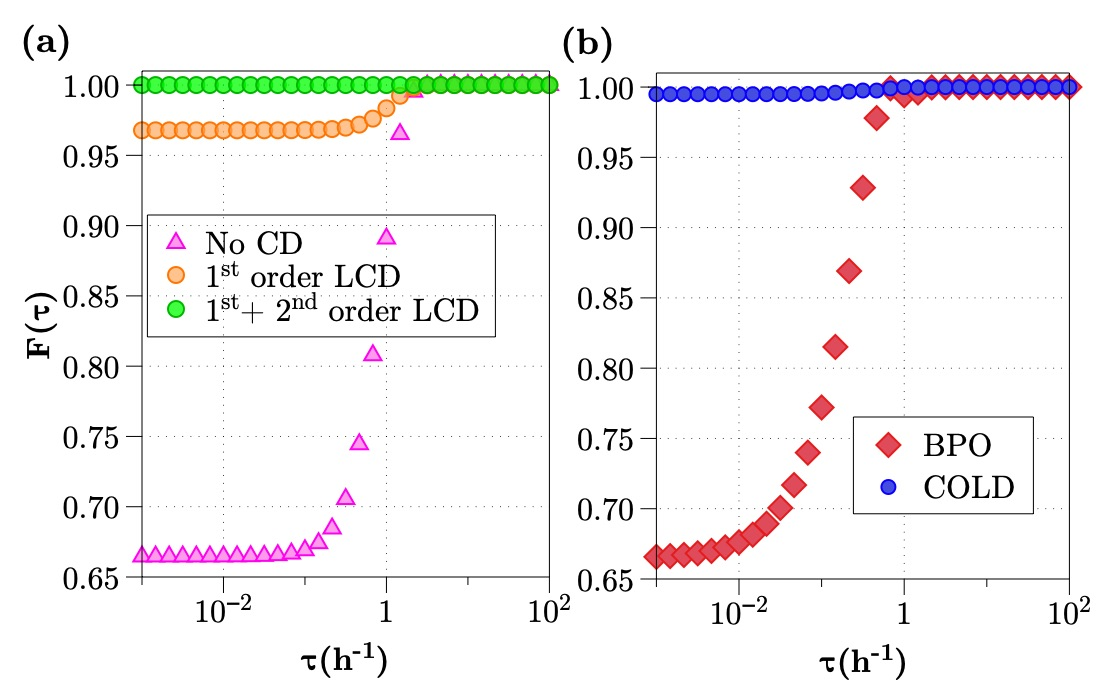
\includegraphics[width=0.8\linewidth]{images/twospins_fidelities.jpg} \caption[COLD applied to two-spin annealing]{}\label{fig:twospin_fidelities}
\end{figure}

\section{Ising chain}\label{sec:5.2_Ising_chain}

\begin{equation}\label{eq:ising_chain_hamiltonian}
    H_0(\lambda) = - J \sum_{j}^{N-1} \sz_j \sz_{j+1} + Z_0\sum_j^N \sz_j + \lambda X_f \sum_j^N \sx_j,
\end{equation}

\begin{equation}
    \AGP{\lambda}^{(1)} = \alpha \sum_{j}^N\sy_j,
\end{equation}

\begin{equation}
    \alpha(\lambda) = \frac{1}{2} \frac{Z_0 X_f}{Z_0^2 + \lambda^2 X_f^2 + 2J^2}.
\end{equation}

\begin{equation}
    \AGP{\lambda}^{(2)} = \alpha \sum_{j} \sy_j + \gamma  \sum_{j} (\sx_j \sy_{j+1} + \sy_j \sx_{j+1}) +  \zeta \sum_{j} (\sz_j \sy_{j+1} + \sy_j \sz_{j+1}) ,
\end{equation}

\section{Transport in a synthetic lattice}

\begin{figure}[t]
    \centering
    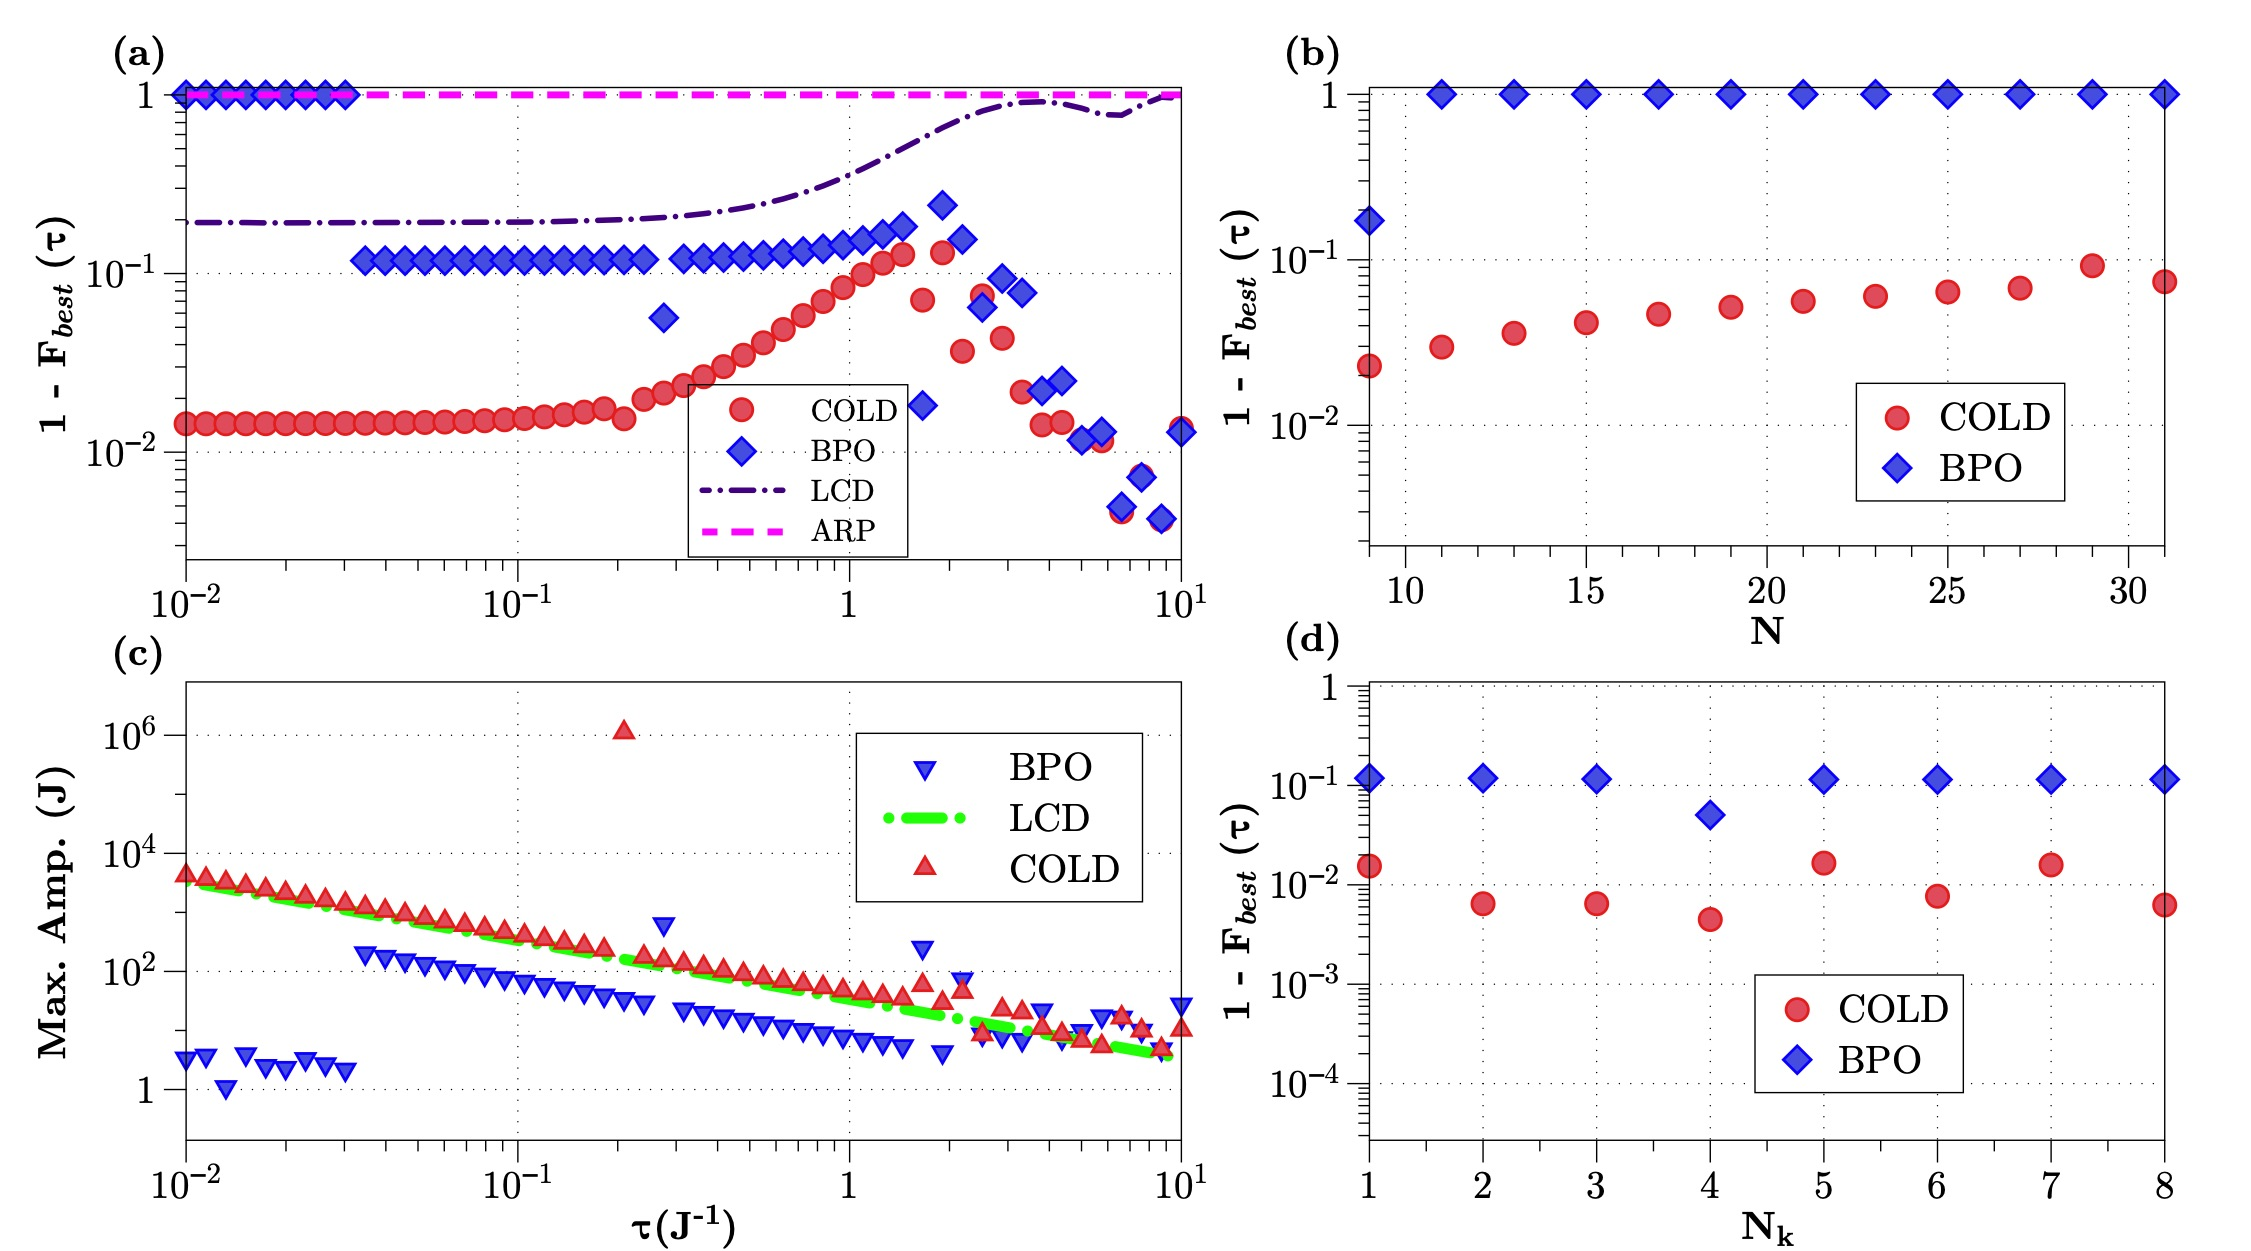
\includegraphics[width=\linewidth]{images/synthetic_lattice.jpg} \caption[COLD plots for ARP transport in a synthetic lattice]{}\label{fig:synthetic_results}
\end{figure}

The efficient transfer of states between opposite ends of a lattice could have future applications in the settings of quantum computation and simulation due to its promise of efficient transport of information \cite{lang_topological_2017}. This objective is often tackled in the setting of ultracold atoms in optical lattices. While the problem can be tuned to be a single-particle system and the analytical solutions of the corresponding instantaneous Schr\"odinger equation are known \cite{hatsugai_chern_1993,hugel_chiral_2014} even for a finite system \cite{duncan_exact_2018}, efficient evolution for state transfer is not straight-forward.  This is due to the fact that the majority of the states are delocalised across the lattice, meaning that the $\ket{\psi}\bra{\psi}$ terms of the CD Hamiltonian of Eq.~\eqref{eq:CD_Hamiltonian} are global in reach. It is common to consider this system in the tight-binding limit where the implementation of global terms is not straightforward. Such terms can be generated via the interactions of the atoms with cavity modes \cite{landig_quantum_2016,keller_phases_2017} or from dipolar interactions \cite{baranov_ultracold_2002, trefzger_ultracold_2011}. However, it would be ambitious to expect this control to be general enough to implement the CD Hamiltonian of the exact solutions.  This is one of the reasons that LCD has been pursued in this setting. 

Recently, LCD has been successfully applied to improve an adiabatic rapid passage (ARP) protocol for population transfer across a synthetic lattice \cite{meier_counterdiabatic_2020}. In this realisation, population transfer was achieved in a synthetic tight-binding lattice of laser coupled atomic momentum states. We will consider the same problem as in Ref.~\cite{meier_counterdiabatic_2020} but with the improvement that can be gained by COLD. This system is described by the Hamiltonian
\begin{equation}\label{eq:lattice_hamiltonian}
    H_0(t) = - \sum_n J_n(t)(c_n^{\dag}c_{n+1} + H.c.) + \sum_n V_n(t) c_n^{\dag}c_n,
\end{equation}

\begin{align} \label{eq:J_lattice}
    J_n(t) &= J_0(1.1 - \lambda) \\ \label{eq:V_lattice}
    V_n(t) &= n V_0 2 (\lambda - 1/2),
\end{align}

\begin{equation}\label{eq:tunneling}
    J_n(t) \rightarrow J_{n, \mathrm{CD}}(t) e^{-i\phi_{n, \mathrm{CD}}(t)},
\end{equation}
where
\begin{align}\label{eq:J_cd}
    J_{n, \mathrm{CD}}(t) = \sqrt{J_n(t)^2 + (\alpha_n(t)/\tau)^2}, \\ \label{eq:phi_cd}
    \phi_{n, \mathrm{CD}}(t)  = \arctan\left(-\frac{J_n(t)\tau}{\alpha_n(t)}\right),
\end{align}

\section{Preparing GHZ states in a system of frustrated spins}\label{sec:6.4_ghz_states}

\begin{figure}[t]
    \centering
    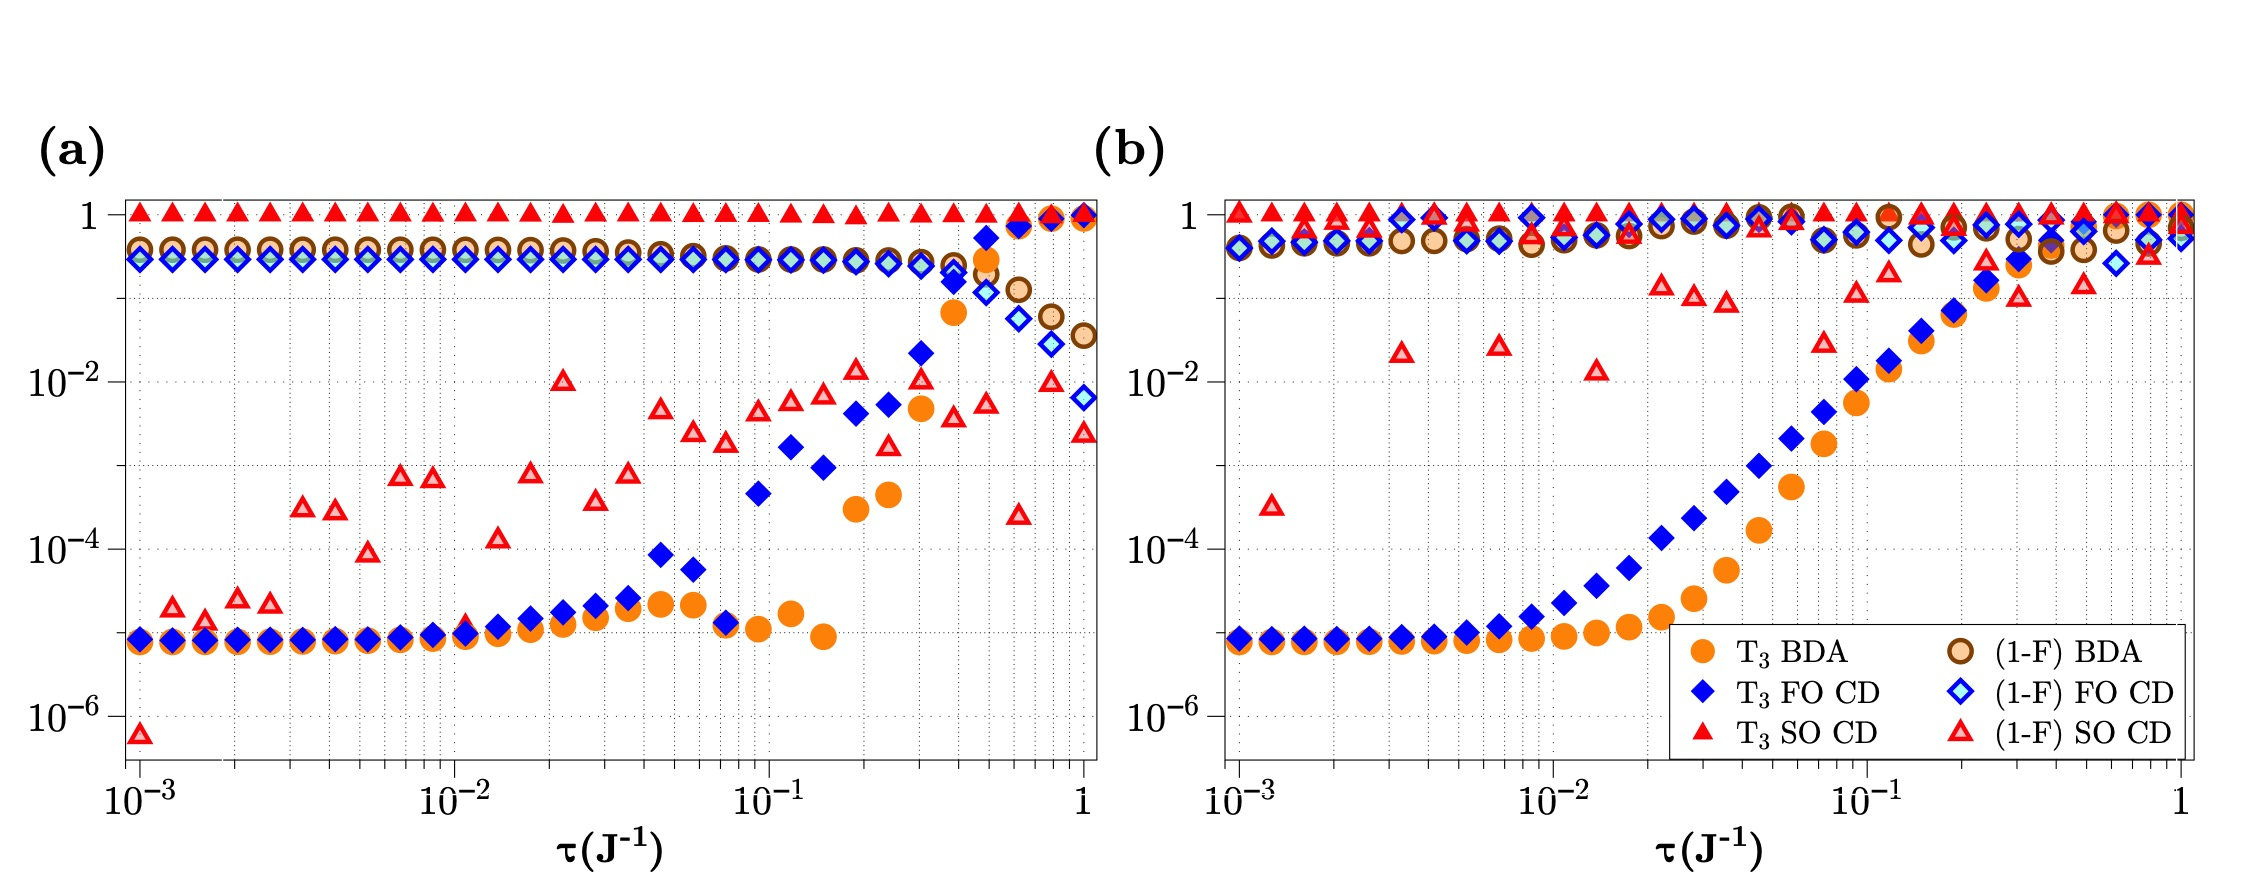
\includegraphics[width=\linewidth]{images/tangle_plots.jpg} \caption[Plots of entanglement and fidelity of GHZ states]{Plots of $T_3$ (Eq.~\eqref{eq:3-tangle}, solid shapes) and fidelity $(1 - F)$ with respect to the GHZ state (outlined shapes) of the final state prepared after optimising a GRAPE pulse with $N_k = 4$ parameters for each value of $\tau$.  (a) Optimisation is performed using $(1 - F)$ as the cost function}\label{fig:tangle_v_fidelity}
\end{figure}

Multipartite entanglement is a powerful resource for quantum computing and more broadly in quantum technologies, offering unique capabilities for information processing, secure communication, high-precision measurements, and understanding the foundations of quantum mechanics. An example of such highly entangled states is the GHZ (Greenberger–Horne–Zeilinger) state \cite{greenberger_bells_1990} on $N > 1$ spins:
\begin{equation}\label{eq:GHZ_state}
    \ket{\rm GHZ} = \frac{1}{\sqrt{2}} (\ket{0}^{\otimes N} + \ket{1}^{\otimes N}).
\end{equation}

\subsection{Tripartite GHZ entanglement}

The GHZ state exhibits a particular type of entanglement: when one of the subsystems is measured, the rest are no longer entangled and collapse into a product state. This is different to the other canonical type of multipartite entanglement exhibited by the W state \cite{cabello_bells_2002}, which for 3 spins can be written as:
\begin{equation}\label{eq:W_state}
    \ket{W} = \frac{1}{\sqrt{3}}(\ket{001} + \ket{010} + \ket{100}).
\end{equation}


GHZ states can be prepared via an annealing schedule on a system of frustrated spins. 

\begin{equation}\label{eq:ghz_hamiltonian}
    H_0(\lambda) = - J \Big( \sum_{j}^{N-1} \sz_j \sz_{j+1} + \sum_{j}^{N-2} \sz_j \sz_{j+2} \Big) - h(1 - \lambda) \Big( \sum_j^N (\sz_j + \sx_j) \Big).
\end{equation}

When $J$ is positive, the ground state of $H_0(1)$ is the GHZ state of Eq.~\ref{eq:GHZ_state}, whereas when it is negative 

While measuring the entanglement of a multipartite system is not quite as simple as in the bipartite case, there exists a notion of entanglement for a system of three spins: namely, the three-tangle, first introduced in Ref.~\cite{coffman_distributed_2000}, which

\begin{equation}\label{eq:3-tangle}
	\begin{aligned}
		T_3(\ket{\psi}) &= 4 \left| d_1 - 2 d_2 + 4 d_3 \right|, \\
		d1 &= c^2_{000}c^2_{111} + c^2_{001}c^2_{110} + c^2_{010}c^2_{101} + c^2_{011}c^2_{100}, \\
		d_2 &= c_{000}c_{001}c_{110}c_{111} + c_{000}c_{010}c_{101}c_{111} + c_{000}c_{011}c_{100}c_{111} \\
		 &+ c_{001}c_{010}c_{101}c_{110} + c_{001}c_{011}c_{100}c_{110} + c_{010}c_{011}c_{100}c_{101} \\
		d_3 &= c_{000}c_{110}c_{101}c_{011} + c_{100}c_{010}c_{001}c_{111}
	\end{aligned}
\end{equation}

Not the first time this is attempted with \acrref{CD}. \cite{sun_optimizing_2022}.

\section{Spin-1/2 XXZ chains of ultracold atoms}

The system is a Mott insulator of $^7$Li atoms in an optical lattice. With one particle per site and two hyperfine states, it realizes the (anisotropic) spin-1/2 Heisenberg model, where effective spin-spin interactions between neighboring sites are realized by a second-order tunneling process (superexchange) \cite{altman03, ddl03}. We apply a microwave field coupling the two hyperfine states with detuning $\delta = \omega - \omega_0$, where $\hbar \omega_0$ is the energy difference between the two hyperfine states and $\omega$ is the frequency of the microwave field, and with Rabi frequency $\Omega$. This is equivalent to having a z- and an x- magnetic field in a spin system respectively, realizing the anisotropic spin-1/2 Hamiltonian with external fields:
\begin{align}
H = & J_z \sum_{\langle i,j \rangle} S_i^zS_j^z+ J_{xy} \sum_{\langle i,j \rangle}  \left(S_i^xS_j^x + S_i^yS_j^y \right) \nonumber \\
& + \delta(\lambda) \sum_i S_i^z + \Omega(\lambda) \sum_i S_i^x,
\label{Heisenberg}
\end{align}